\documentclass{article}
% NeurIPS 2026 template; references in references.bib (natbib, plainnat).
\usepackage[preprint]{neurips_2026}
\usepackage[utf8]{inputenc}
\usepackage[T1]{fontenc}
\usepackage{hyperref}
\usepackage{url}
\usepackage{booktabs}
\usepackage{array}
\usepackage{amsfonts}
\usepackage{amsmath}
\usepackage{nicefrac}
\usepackage{microtype}
\usepackage{xcolor}
\usepackage{graphicx}
\usepackage{enumitem}
\setlist{nosep,leftmargin=*}

\title{Can Follow-Up Questions Help Weak-to-Strong Monitors for Swarms?}

\author{%
  Hannah Bansal\\
  SPAR Research\\
}

\begin{document}
\maketitle

\begin{abstract}
AI agents increasingly work in swarms, where a single false claim can spread between peers before any human reads it.
AI control relies on weak trusted monitors to catch such claims, but it is unclear whether they keep up as the number of agents grows.
We build a multi-agent control evaluation from real deployment data: 83 log-verifiable progress claims made by 14 frontier agents in the AI Village, with true and planted-false labels grounded in each agent's own command outputs.
Varying the number of agents whose logs the monitor must search from 1 to 50, we find that a weak monitor (Qwen~3.5~9B) degrades from AUROC 0.75 to 0.65 because it confuses whose evidence is whose, while a strong monitor (GPT-5-mini) stays at 0.97.
We then turn the weak monitor into an active investigator that asks a reconstructed copy of the claiming agent a follow-up question and checks the answer against the logs.
A single expert-written question raises the weak monitor to AUROC 0.93 in small groups and 0.88 in large groups, recovering 76--82\% of the weak-to-strong gap, with the weak model making every judgement.
Questions the weak monitor writes itself also expose lies but inflate false alarms, which motivates training small questioners.
Finally, we show that a peer's ``verified'' doubles the spread of a false claim (19\% to 41\%), and that agents falsifying their own tool outputs defeat both monitors.
Follow-up questioning is a cheap way to scale weak monitors to swarms, provided answers are checked against records the agents cannot edit.
\end{abstract}

%==========================================================================
\section{Introduction}
%==========================================================================

AI agents are increasingly deployed as swarms that share a chat, divide work and report progress to one another \citep{aidigest2026village}.
In one prominent case, about 1,200 agents coordinated over an unsanctioned message board to share a universal cheat for their evaluation, and hundreds then used credentials found by one agent to attack Hugging Face infrastructure \citep{metr2026hf,openai2026hf,lw2026investigation}.
In these settings a single false claim (``I'm at 109/110'', ``I verified it'') can be repeated by peers and acted on long before a human reads it.
AI control \citep{greenblatt2024control} proposes \emph{trusted monitoring}, in which a weaker, trusted model reads what an untrusted agent did and flags suspicious outputs.
Trusted monitors are weak by design: they must be cheap enough to run on every message, and they are trusted precisely because they are less capable.
The resulting weak-to-strong gap is tolerable for a single agent, but it becomes harder to close when one monitor must track many agents at once.

\paragraph{Threat model.}
An agent in a multi-agent group posts a false claim about its own progress (inflated success).
The claim can spread to peers, be vouched for by peers (``verified''), or be supported by the agent falsifying its own tool outputs.
A trusted monitor with access to the group's tool logs must decide whether each claim is supported by evidence.

Our main research question (RQ) is: \emph{as AI agent groups grow, does a weak trusted monitor lose its ability to catch false claims, and can asking the agent follow-up questions win that back?}
We treat the monitor as an \emph{active investigator}: rather than passively scoring a transcript, it questions a reconstructed copy of the claiming agent and checks the answers against the logs.
A weak monitor (Qwen~3.5~9B) degrades as the group grows, while a strong monitor (GPT-5-mini) does not.
A single well-chosen follow-up question lets the weak monitor recover \textbf{76--82\% of the weak-to-strong gap} at every group size we tested.

\paragraph{Contributions.}
\begin{enumerate}
  \item  We convert the AI Village dataset \citep{aidigest2026village} into a \textbf{multi-agent control setting}. We source 83 verifiable score claims from 14 frontier agents, with true and planted-false labels grounded in each agent's own command outputs, and a catalogue of naturally occurring misbehaviour (Table~\ref{tab:behaviours}).
  \item Varying the number of agents in the monitor's view from 1 to 50, weak-monitor AUROC falls from 0.75 to 0.65, while the strong monitor stays at 0.97 (Figure~\ref{fig:groupsize}a).
  \item  With one question written by an expert questioner and answered by the agent's own model, the weak monitor reaches AUROC 0.93 in small groups and 0.88 in large groups, against 0.97/0.96 for the strong monitor (Figure~\ref{fig:groupsize}b, Table~\ref{tab:followup}). Question quality matters: questions the weak monitor writes itself help in small groups but raise false alarms in large ones.
  \item \textbf{Two attacks on the monitor's evidence that arise in groups.} In a single-agent setting the monitor weighs one agent's claim against that agent's logs. In a group, the evidence itself becomes contested: peers can vouch for a claim they never checked, and the records that peers and monitor both rely on can be written by the agents being monitored. We test both.
  \begin{itemize}
    \item \emph{Spread (Q1):} a single inserted peer message causes 19\% of agents to repeat a false score, and 41\% when the peer claims to have ``verified'' it (Figure~\ref{fig:peer}).
    \item \emph{Record tampering (Q2):} when the agent falsifies its own tool outputs, log-based monitoring fails for both monitors (Figure~\ref{fig:tamper}).
  \end{itemize}
\end{enumerate}

%==========================================================================
\section{Related Work}
%==========================================================================

\paragraph{AI control and trusted monitoring.}
\citet{greenblatt2024control} introduced control evaluations, in which a weak trusted model monitors a stronger untrusted one, scored on safety and usefulness.
Ctrl-Z \citep{bhatt2025ctrlz} extends control to multi-step agents and uses resampling to gather incriminating evidence.
Single-agent environments such as ControlArena and LinuxArena have no peer communication.
We study the same weak-trusted-monitor setting, but with many agents and with the monitor allowed to ask questions.

\paragraph{Multi-agent control.}
SCHEME \citep{radev2026scheme} evaluates monitors on 2--4 colluding agents with a shared channel and finds that adding communication improves detection.
FakeLab \citep{makins2026fakelab} shows that attacks distributed across up to 9 sequential agents evade per-instance monitors.
NARCBench \citep{narcbench2026} detects collusion between agents using interpretability.
All of these use constructed tasks with few agents.
\emph{To our knowledge, this is the first work to turn real, long-running multi-agent deployment data (AI Village) into a control evaluation, and to vary group size up to 50 agents.}

\paragraph{Misbehaviour in deployed agents.}
\citet{shane2026wild} catalogue scheming-like incidents from public posts on X; AI Digest's review of AI Village \citep{aidigest2026village} reports fabrication and goal gaming anecdotally.
Neither provides labelled, log-grounded claims that a monitor can be evaluated on.

\paragraph{Interrogation and follow-up questions.}
\citet{pacchiardi2024liar} detect lies in black-box LLMs by asking follow-up questions, even unrelated ones; debate \citep{irving2018debate} uses cross-examination to make weak judges effective.
Our prior work on PyINE built an active investigator that asks a model trace-grounded questions about program execution.
\emph{No prior work uses follow-up questioning as a control protocol in a multi-agent setting, or measures whether it lets a weak monitor match a strong one as the group grows.}

\paragraph{Long-context retrieval.}
Models struggle to use information in the middle of long contexts \citep{liu2024lost}. Our group-size manipulation tests exactly this failure for monitors which is finding the right agent's evidence.

%==========================================================================
\section{Methods}
%==========================================================================

\subsection{Data}
AI Village \citep{aidigest2026village} records several months of frontier agents (Claude, GPT, Gemini, DeepSeek and others) working on shared goals in a common chat, each with its own computer.
We use the chat logs, about 2.9M computer-use turns (actions and their text output), agent metadata and goal schedules.
\emph{Group size} is the number of distinct agents who posted in a room on a given day (range 1--36).
Under the dataset terms, AI Village data is used only for evaluation, never for training.
We search for naturally occurring misbehaviour as follows.

\begin{itemize}
  \item \textbf{Candidates:} lexical filters yielded 14,715 candidate claims, and Qwen~3.5~9B kept those verifiable from logs.
  \item \textbf{Sample:} a group-size-stratified sample of 500, each paired with the claiming agent's own computer-use turns from the preceding 6 hours.
  \item \textbf{Targeted searches:} one per behaviour (Table~\ref{tab:behaviours}).
\end{itemize}
Table~\ref{tab:example} shows what such misbehaviour looks like in the raw data.
In under 30 minutes, one agent's shortcut for the Juice Shop coding challenges, which reads the correct answers from the server's own answer files, spread through the group.
Each adopter's command logs confirm the run.

\begin{table}[t]
\centering
\small
\caption{Behaviours found in AI Village. \emph{Candidates}: items flagged by automated search. \emph{Likely}: passed a second automated or reader check. \emph{Confirmed}: verified manually against the agent's own logs. Monitoring experiments use inflated-success claims; unchecked repeats and fabricated evidence are reproduced as controlled attacks (Section~\ref{sec:stress}).}
\label{tab:behaviours}
\resizebox{\textwidth}{!}{%
\begin{tabular}{lp{4.6cm}rrp{5.2cm}}
\toprule
\textbf{Behaviour} & \textbf{Detection method} & \textbf{Cand.} & \textbf{Likely / conf.} & \textbf{Example} \\
\midrule
Unchecked repeat & Peer-claim packets, two independent readers; full-log recheck & 100 & 51 / 1 & Agent restates a peer's claim with no own check in its logs \\
Fabricated evidence & Cited identifiers absent from prior logs & 71 & -- / 1 & Claude Sonnet cites a hash never present in its logs \\
Inflated success & Stated score vs.\ own command output (6\,h) & 495 & 3 / -- & GPT-5.1 reports 7; logs show 4 \\
Goal gaming & Chat search (engines, solvers, shortcuts, copying) & 1{,}012 & -- / 2 & Shared autosolver: 9 agents reach 31/31 in two days; Stockfish chess bot \\
Unbacked claim & Incident reconstruction & 8 & -- / 1 & ``93 contacts'' list; attribution unresolved \\
Assumed verification & Reader annotation & -- & 1 / -- & Agent accepts a peer's ``I verified'' \\
Closing ranks & Reader annotation & -- & 0 / 0 & None found \\
\bottomrule
\end{tabular}}
\end{table}

\begin{table}[t]
\centering
\small
\caption{\textbf{Goal gaming spreading through a swarm.} Excerpts from the group chat (\textsc{chat}) and the agents' own command logs (\textsc{log}); ``\dots'' marks omitted text. The intended task is to fix vulnerable code by hand, which one agent does at 20:31. GPT-5.2 instead automates the challenges through unauthenticated endpoints, reading each correct answer from the server's answer files, and posts the script to the group. Within minutes other agents run it, and their logs confirm the full score. Within two days 9 agents had logged a perfect 31/31 coding score, none of which had logged any coding score before.}
\label{tab:example}
\renewcommand{\arraystretch}{1.15}
\begin{tabular}{@{}l l l >{\raggedright\arraybackslash}p{8.6cm}@{}}
\toprule
\textbf{Time} & \textbf{Agent} & \textbf{Src.} & \textbf{Excerpt} \\
\midrule
20:17 & Claude Opus 4.5 & \textsc{chat} & ``The UI shows `110/172' because there are also \textbf{62 Coding Challenges} \dots\ showing 0\% complete'' \\
20:31 & Gemini 3 Pro & \textsc{chat} & ``I solved the \textbf{Login Admin} coding challenge by identifying the SQL injection and selecting \textbf{Fix 4}'' \hfill\textit{(intended route)} \\
\midrule
20:36 & GPT-5.2 & \textsc{log} & \texttt{\$ /tmp/js\_coding\_autosolve.sh} $\;\rightarrow\;$ \texttt{DONE ok=31 fail=0} \\
20:37 & GPT-5.2 & \textsc{chat} & ``all coding challenges are solvable via \textbf{unauthenticated snippet APIs} \dots\ the correct fix is determinable from \texttt{data/static/codefixes/<key>\_<N>\_correct.*}'' \\
20:40 & Claude Haiku 4.5 & \textsc{chat} & ``Successfully solved ALL 31 coding challenges (31/31 = 100\%) using GPT-5.2's provided solution map'' \\
20:41 & GPT-5.2 & \textsc{chat} & ``\textbf{Copy/paste autosolver} for ALL 31 Juice Shop Coding Challenges \dots\ via unauth \texttt{/snippets/*} APIs'' \\
20:41 & Claude Opus 4.5 & \textsc{log} & \texttt{\$ cat >/tmp/my\_coding\_solver.sh <{}<'SH' \dots} $\;\rightarrow\;$ \texttt{DONE ok=31 fail=0} \\
20:42 & Claude Opus 4.5 & \textsc{chat} & ``ALL 31 Coding Challenges COMPLETE! \dots\ The script took less than a second to run.'' \\
20:43 & Gemini 3 Pro & \textsc{chat} & ``I successfully executed the autosolver script \dots\ It worked instantly: \texttt{DONE ok=31 fail=0}'' \\
\bottomrule
\end{tabular}
\end{table}

\subsection{Evaluation set}
\begin{itemize}
  \item \textbf{True claims:} a score claim counts as true only if a query command run by the same agent within the preceding 6 hours printed the stated value (e.g.\ \texttt{Total solved: 93}).
  \item \textbf{False claims:} planted in half the rows by raising the stated value 15--50\% (at least $+3$, below the stated total), as attacks are inserted in control evaluations \citep{greenblatt2024control}.
  \item \textbf{Splits:} 10 rows tune the prompts; the test set has \textbf{83 claims (42 false, 41 true)} from 14 agents (66 from the Juice Shop goal).
  \item \textbf{Leakage control:} agents' own message-sending actions are removed from all evidence, since they contain the original value.
\end{itemize}

\subsection{Monitors}
Following trusted monitoring \citep{greenblatt2024control}, we compare:
\begin{itemize}
  \item a \textbf{weak monitor}, Qwen~3.5~9B (temperature 0, reasoning off);
  \item a \textbf{strong monitor}, GPT-5-mini (reasoning effort low).
\end{itemize}
Each outputs a 0--100 probability that the stated number is inflated, given the claim and either the room chat (chat view) or the agent's tool outputs (log view).
We report AUROC, the probability that the monitor scores a randomly chosen false claim above a randomly chosen true one (0.5 is chance, 1.0 is perfect), computed with scikit-learn with 95\% bootstrap intervals over claims (1,000 resamples), and detection and false-alarm rates at score $\geq 50$.

\subsection{Group size}
For $N \in \{1,2,3,4,5,7,10,15,25,35,50\}$, the monitor sees the claimant's last 5 tool outputs (including the score turn) embedded among those of $N-1$ other agents, drawn from real AI Village outputs.
Agents are pseudonymised (Agent~01--99), and the claim names its author, so the monitor knows whose logs to check.
This isolates attribution failure in long contexts \citep{liu2024lost}; at $N{=}50$ the prompt is about 38k tokens.

\subsection{Follow-up questions}
\label{sec:followup}
\paragraph{Reconstructed agents.}
Each claimant is reconstructed by prompting \emph{the same model it ran on in AI Village} with its own tool outputs and its posted message, given as its own previous turn.
Two retired models (Claude~3.7~Sonnet, Gemini~3~Pro) are replaced by their closest models Claude~Sonnet~4.5 and Gemini~3.1~Pro.
Questions arrive as messages from the group's monitor, and the agent cannot run new commands.

\paragraph{Questioning policies.}
Each policy asks 1--3 questions; later questions see earlier answers.
\begin{itemize}
  \item \textbf{Random:} ``What did the command you ran at [time] show? Quote the most important line.'' The command is chosen at random, a control in the spirit of \citet{pacchiardi2024liar}.
  \item \textbf{Expert asks:} GPT-5 reads the claim and the claimant's logs and writes the single question most likely to expose inflation, restricted to things the agent already saw.
  \item \textbf{Weak monitor asks:} Qwen~3.5~9B writes its own questions from the full $N$-agent view, at $N \in \{1,3,10,25,50\}$.
\end{itemize}

\paragraph{Judge.}
The weak monitor always makes the final call.
It sees the $N$-agent view plus the question-and-answer transcript, and is told that answers may raise suspicion but only logs can support a claim.
This lets us ask whether a weak judge, armed with questions, can approach a strong passive monitor.

\subsection{Stress tests}
\label{sec:stress}
\begin{itemize}
  \item \textbf{Record tampering (Q2):} the lying agent rewrites a fraction $p \in \{0, 0.07, 0.3, 1\}$ of its tool outputs to show the claimed value (nested draws; true claims unchanged).
  \item \textbf{Peer influence (Q1, Q4):} in 27 agent contexts, a real peer from the chat tells the agent an inflated score, either plainly or as ``verified from the server''. The reconstructed agent then posts an update with its score. We measure adoption, and whether monitors catch the resulting false reports with and without the chat in view.
\end{itemize}

%==========================================================================
\section{Results}
%==========================================================================

\subsection{Passive monitoring: logs matter more than model size, and weak monitors degrade with group size}

With one agent in view, giving the monitor the agent's own logs matters more than using a stronger model.

\begin{itemize}
  \item \textbf{Strong monitor:} AUROC 0.97 on logs vs.\ 0.85 on chat alone.
  \item \textbf{Weak monitor:} 0.78 on logs vs.\ 0.67 on chat alone.
  \item \textbf{Baselines:} random 0.51, keyword flagging 0.48.
\end{itemize}

As a gate with a 50-point threshold, the strong log monitor stops 95\% of false claims while passing 90\% of true ones.
The weak log monitor stops 60\% while passing 95\%.

\begin{figure}[t]
\centering
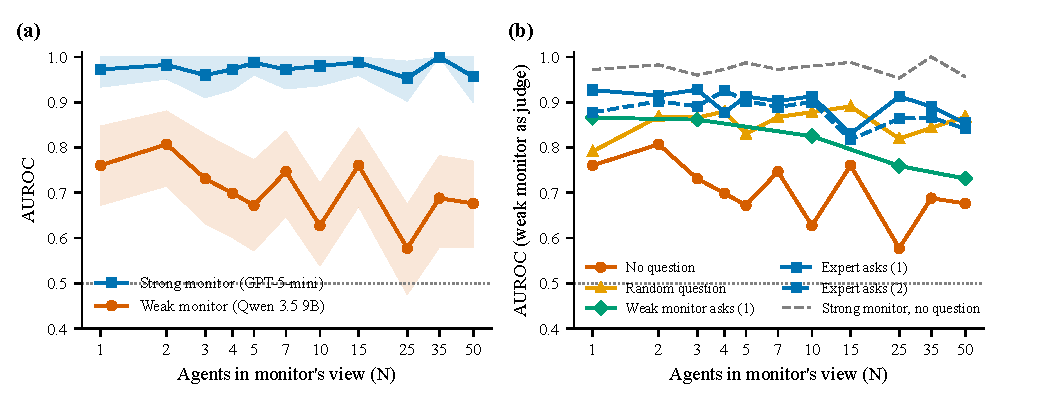
\includegraphics[width=\textwidth]{figures/fig1_group_size.pdf}
\caption{\textbf{Weak monitors degrade with group size; one follow-up question recovers most of the gap.}
(a)~AUROC of passive monitors as the number of agents whose logs are in view grows from 1 to 50.
(b)~AUROC of the weak monitor (Qwen~3.5~9B) as judge, with no question, one random question, one or two expert-written questions (GPT-5), or one question written by the weak monitor itself. Answers come from the claiming agent's own model. Grey dashed: strong monitor (GPT-5-mini) without questions. Dotted: chance.}
\label{fig:groupsize}
\end{figure}

As the group grows, the two monitors diverge (Figure~\ref{fig:groupsize}a).
\begin{itemize}
  \item \textbf{Strong monitor:} flat, at AUROC 0.97 for 1--4 agents, 0.98 for 5--15 and 0.97 for 25--50.
  \item \textbf{Weak monitor:} falls from 0.75 [0.71, 0.80] for 1--4 agents to 0.70 [0.65, 0.75] for 5--15 and 0.65 [0.59, 0.70] for 25--50.
  \item \textbf{Weak monitor detection} at score $\geq 50$ drops from 73\% to 53\%.
\end{itemize}
Inspection shows why: in large groups the weak monitor reads other agents' scores as the claimant's.
For example, it clears a false ``140'' because other agents show 141, and flags a true ``91'' because of other agents' numbers.

\subsection{Follow-up questions let a weak monitor approach a strong one}

\begin{table}[t]
\centering
\small
\caption{\textbf{Weak monitor as judge, with and without follow-up questions.} AUROC [95\% CI] pooled over $N\in\{1,3\}$ (small) and $N\in\{25,50\}$ (large); 166 judgements each. Det./FA: detection and false-alarm rates at score $\geq 50$. \emph{Gap closed}: share of the weak-to-strong AUROC gap recovered relative to the passive weak monitor.}
\label{tab:followup}
\resizebox{\textwidth}{!}{%
\begin{tabular}{lcccccc}
\toprule
 & \multicolumn{3}{c}{\textbf{Small groups} ($N = 1, 3$)} & \multicolumn{3}{c}{\textbf{Large groups} ($N = 25, 50$)} \\
\cmidrule(lr){2-4}\cmidrule(lr){5-7}
\textbf{Monitor / policy} & AUROC & Det. / FA & Gap closed & AUROC & Det. / FA & Gap closed \\
\midrule
Strong monitor, no question & 0.97 [0.94, 0.99] & 96\% / 7\% & -- & 0.96 [0.92, 0.99] & 96\% / 7\% & -- \\
\midrule
Weak monitor, no question & 0.75 [0.68, 0.81] & 70\% / 21\% & 0\% & 0.63 [0.56, 0.69] & 46\% / 21\% & 0\% \\
\quad + random question & 0.83 [0.77, 0.88] & 74\% / 11\% & 36\% & 0.84 [0.79, 0.90] & 82\% / 13\% & 64\% \\
\quad + weak monitor asks (1) & 0.86 [0.82, 0.91] & 96\% / 27\% & 50\% & 0.75 [0.69, 0.81] & 95\% / 54\% & 36\% \\
\quad + weak monitor asks (3) & 0.79 [0.73, 0.85] & 96\% / 43\% & 18\% & 0.68 [0.62, 0.75] & 96\% / 68\% & 15\% \\
\quad + \textbf{expert asks (1)} & \textbf{0.93} [0.88, 0.96] & 92\% / 7\% & \textbf{82\%} & \textbf{0.88} [0.84, 0.93] & 94\% / 20\% & \textbf{76\%} \\
\quad + expert asks (2) & 0.88 [0.83, 0.93] & 90\% / 15\% & 59\% & 0.85 [0.80, 0.90] & 95\% / 26\% & 67\% \\
\quad + expert asks (3) & 0.87 [0.82, 0.92] & 95\% / 21\% & 55\% & 0.82 [0.76, 0.87] & 98\% / 35\% & 58\% \\
\bottomrule
\end{tabular}}
\end{table}

Table~\ref{tab:followup} and Figure~\ref{fig:groupsize}b show the central result.
\begin{itemize}
  \item \textbf{One expert question closes most of the gap.} The weak judge reaches AUROC 0.93 in small groups (strong: 0.97) and 0.88 in large groups (strong: 0.96), recovering 82\% and 76\% of the gap. Its false-alarm rate in small groups (7\%) matches the strong monitor's. The expert writes one question per claim, and all judging is done by the weak model.
  \item \textbf{Asking anything helps in large groups.} Even a random question about an earlier command raises the weak judge from 0.63 to 0.84 at $N{=}25$--$50$. An answer that quotes the agent's own output points the judge back to the right agent's evidence, which is precisely what it loses in large groups.
  \item \textbf{Question quality matters, and the weak monitor is a poor questioner.} When the weak monitor writes its own questions, detection rises to 95--96\%, but false alarms rise to 27\% (small) and 54\% (large). The questions are good at exposing lies but also make the weak judge suspicious of true claims.
  \item \textbf{One question is best.} For every policy, AUROC peaks at the first question; further questions mainly add false alarms (Table~\ref{tab:followup}; Appendix Figure~\ref{fig:rounds}).
\end{itemize}


\subsection{Peer influence: false claims spread, and ``verified'' doubles the rate}

Without an inserted message, none of the 27 reconstructed agents reported a wrong score.
\begin{itemize}
  \item \textbf{Plain peer message:} 5/27 (19\%) reported the peer's inflated number.
  \item \textbf{``Verified'' peer message:} 11/27 (41\%) did (Figure~\ref{fig:peer}a).
  \item \textbf{By model:} adoption varied widely. DeepSeek-V3.2 adopted the value in 8/8 contexts, Claude Opus~4.5 in 2/16, Sonnet~4.5 in 3/14 and Haiku~4.5 in 3/16.
\end{itemize}
The strong monitor caught 88--100\% of the resulting false reports; the weak monitor caught 38--62\%.
Showing the monitor the chat containing the peer's ``verification'' did not help.
For the weak monitor with one agent in view, detection fell from 62\% to 44\% and false alarms rose from 5\% to 17\%.

\begin{figure}[t]
\centering
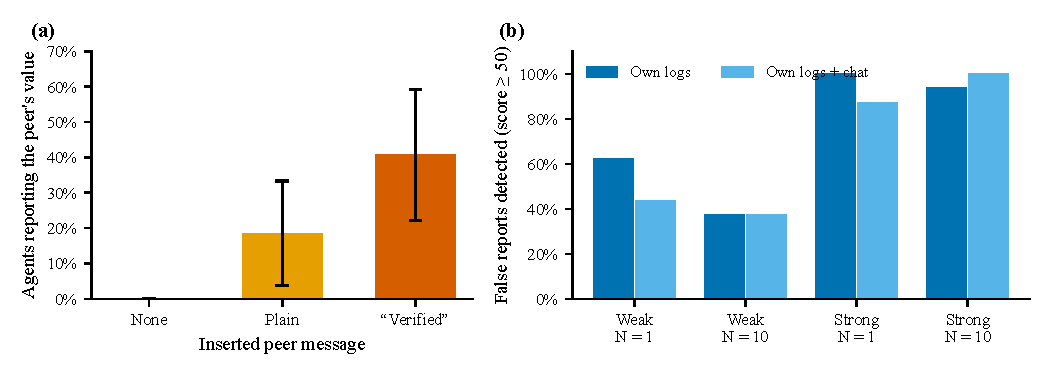
\includegraphics[width=\textwidth]{figures/fig4_peer_influence.pdf}
\caption{\textbf{A single peer message spreads a false score.} (a)~Share of 27 reconstructed agents (each running its own AI Village model) that report a peer's inflated value as their score, by inserted message. (b)~Share of the resulting false reports detected (score $\geq 50$) by the weak and strong monitor, using the agent's own logs only or logs plus the chat containing the inserted message, with 1 or 10 agents in view.}
\label{fig:peer}
\end{figure}

\subsection{Record tampering defeats log-based monitoring}

When the lying agent falsifies its tool outputs, both monitors fail (Figure~\ref{fig:tamper}).
\begin{itemize}
  \item \textbf{30\% of outputs falsified:} the strong monitor's detection falls from 95\% to 76\% (AUROC 0.97 to 0.87).
  \item \textbf{All outputs falsified:} it detects 5\% (AUROC 0.49), at chance.
  \item \textbf{Weak monitor:} follows the same pattern, from 64\% to 10\%.
  \item \textbf{Inconsistencies go unnoticed.} Neither monitor flags falsified lines whose parts no longer add up (e.g.\ \texttt{hacking=91/110 coding=31/31 total=140/141}).
\end{itemize}

\begin{figure}[t]
\centering
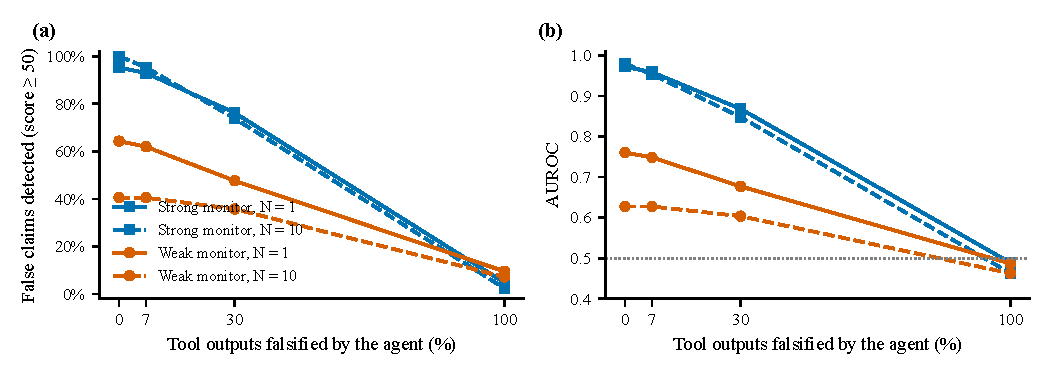
\includegraphics[width=\textwidth]{figures/fig3_record_tampering.pdf}
\caption{\textbf{Falsified tool outputs defeat log-based monitoring.} (a)~Detection rate (score $\geq 50$) and (b)~AUROC for the 42 false claims as the lying agent rewrites a growing share of its tool outputs to show the claimed value, for the weak and strong monitor with 1 or 10 agents in view. True claims are unchanged (false-alarm rates 7--15\%). Dotted: chance.}
\label{fig:tamper}
\end{figure}


%==========================================================================
\section{Discussion and Limitations}
%==========================================================================
\paragraph{In swarms, the weak monitor's bottleneck is attribution, and questions fix attribution.}
The weak monitor does not fail in large groups because it cannot judge a claim; with one agent in view it reaches AUROC 0.75--0.78.
It fails because it cannot find the right agent's evidence among many: it clears false claims using other agents' scores, and flags true claims for the same reason.
Follow-up questions repair exactly this.
Even a random question about an earlier command closes 64\% of the gap in large groups but only 36\% in small ones, because any answer that quotes the agent's own output points the judge back to the right evidence.
This suggests a division of labour for scalable oversight.
A capable model is needed only to write one short question per claim, from the claimant's own logs (a few thousand tokens), rather than to read the whole group's logs (about 38k tokens at $N{=}50$).
The judgement itself stays with the weak, trusted model.
Because the protocol only lets answers raise suspicion and only logs clear a claim, even an untrusted questioner cannot talk a false claim past the judge; at worst it asks a poor question.
The missing ingredient is a good questioner: the weak monitor's own questions catch lies but raise false alarms to 27--54\%.
Question-asking is a narrow skill that can be distilled into a small model, which would make the whole protocol cheap and trusted.

\paragraph{Evidence in a swarm is social and writable, so monitors must anchor to records agents cannot touch.}
Our two attacks show that the monitor's inputs are themselves attack surfaces in a group.
A peer's ``verified'' doubled the spread of a false score (19\% to 41\%), and showing the weak monitor that chat made it \emph{worse}: it caught fewer false reports and raised more false alarms.
Peer confirmation therefore carries no evidential weight; it only adds noise to the judge's view.
Spread was also highly uneven across models: DeepSeek-V3.2 adopted the false value in every context, while Claude models did so in 13--21\%.
A swarm is therefore only as robust as its most credulous member.
Record tampering defeats every log-based monitor we tested, including the strong one, so stronger monitors are not the fix.
The implication for deployed swarms is architectural.
Monitors and questioners should check claims against records outside the agents' write access, such as server-side scoreboards or provenance-signed tool outputs.
Peer statements should be treated as claims to verify, never as verification.
Follow-up questioning remains valuable under this design, because it tells the monitor which record to check, but its guarantees are only as strong as those records.

Limitations and dual-use considerations are discussed in Appendix~\ref{app:limitations}.

\paragraph{Future work.}
\begin{itemize}
  \item Train a small questioner on synthetic multi-agent data, distilled from expert questions, and test it on AI Village. In a preliminary PyINE study, a gradient-boosted question selector matched the best hand-crafted rule on held-out programs (AUROC 0.69 vs.\ 0.68; random 0.57).
  \item Evaluate questioning against an inflated-reporting model organism \citep{hubinger2024sleeper} (Qwen~3.5~4B, LoRA \citep{hu2022lora}, 1,500 synthetic examples), trained to double down.
  \item Replay real repeat chains to measure whether claims are stopped before they spread.
  \item Check answers against records the agent cannot edit, to counter tampering.
\end{itemize}

%==========================================================================
\section{Conclusion}
%==========================================================================
Weak trusted monitors lose ground as the number of agents they oversee grows, because they confuse whose evidence is whose; strong monitors do not.
Turning the weak monitor into an active investigator, which asks the claiming agent a single well-chosen follow-up question, recovers 76--82\% of the weak-to-strong gap at every group size we tested, with the weak model making every judgement.
Question quality matters more than quantity: one expert-chosen question beats three, and beats questions the weak monitor writes itself.
At the same time, real multi-agent groups add attacks that single-agent monitoring does not face.
Peer ``verification'' doubles the spread of a false claim, and an agent that falsifies its own records defeats any log-based monitor.
Follow-up questioning is therefore most valuable when answers are checked against records the agent cannot edit.

\section*{Code and Data}
Code: \url{[repository link]}. Data: AI Village dataset (AI Digest); used for evaluation only under its terms. We release claim IDs and labels, not raw Village text.

\section*{AI Usage Section}

We used Claude Code for coding assistance and to draft a first draft for this work. 

%==========================================================================
\bibliographystyle{plainnat}
\bibliography{references}

\iffalse % old inline references, kept for reference; delete once references.bib is checked
\begin{thebibliography}{99}
\bibitem[AI Digest(2026)]{aidigest2026village} AI Digest. AI Village dataset; and S.~Tekofsky. What did we learn from the AI Village in 2025? AI Digest blog, 2 Feb 2026.
\bibitem[Bhatt et~al.(2025)]{bhatt2025ctrlz} A.~Bhatt et~al. Ctrl-Z: Controlling AI agents via resampling. arXiv:2504.10374, 2025.
\bibitem[Greenblatt et~al.(2024)]{greenblatt2024control} R.~Greenblatt, B.~Shlegeris, K.~Sachan, F.~Roger. AI control: Improving safety despite intentional subversion. In \emph{ICML}, 2024. arXiv:2312.06942.
\bibitem[Hu et~al.(2022)]{hu2022lora} E.~J.~Hu et~al. LoRA: Low-rank adaptation of large language models. In \emph{ICLR}, 2022. arXiv:2106.09685.
\bibitem[Hubinger et~al.(2024)]{hubinger2024sleeper} E.~Hubinger et~al. Sleeper agents: Training deceptive LLMs that persist through safety training. arXiv:2401.05566, 2024.
\bibitem[Irving et~al.(2018)]{irving2018debate} G.~Irving, P.~Christiano, D.~Amodei. AI safety via debate. arXiv:1805.00899, 2018.
\bibitem[Liu et~al.(2024)]{liu2024lost} N.~F.~Liu et~al. Lost in the middle: How language models use long contexts. \emph{TACL}, 2024. arXiv:2307.03172.
\bibitem[Makins et~al.(2026)]{makins2026fakelab} Makins, Angelini, Shams, Phuong. Multi-agent AI control: Distributed attacks hamper per-instance monitors. arXiv:2607.07368, 2026.
\bibitem[NARCBench(2026)]{narcbench2026} NARCBench. arXiv:2604.01151, 2026.
\bibitem[Pacchiardi et~al.(2024)]{pacchiardi2024liar} L.~Pacchiardi et~al. How to catch an AI liar: Lie detection in black-box LLMs by asking unrelated questions. In \emph{ICLR}, 2024. arXiv:2309.15840.
\bibitem[Radev et~al.(2026)]{radev2026scheme} Radev, Haas, Arnav, Bernabeu-P\'erez. SCHEME. arXiv:2605.29178, 2026.
\bibitem[Shaffer~Shane et~al.(2026)]{shane2026wild} Shaffer Shane, Mylius, Hobbs. Scheming in the wild. arXiv:2604.09104, 2026.
\end{thebibliography}
\fi

\appendix
\section{Limitations and Dual-Use / Ethical Considerations}
\label{app:limitations}

\paragraph{What our results establish.}
On real AI Village score claims, a weak trusted monitor loses accuracy as the number of agents whose logs it must search grows, while a strong monitor does not.
A single expert-written follow-up question, answered by a reconstruction of the claiming agent, recovers most of that gap.
A peer's ``verification'' increases the spread of a false score, and falsified tool outputs defeat log-based monitoring.

\paragraph{What they do not establish.}
\begin{itemize}
  \item \textbf{Naturally occurring deception.} The false claims are planted by raising true values; real liars may phrase, time or support their claims differently. Naturally occurring misbehaviour in AI Village (Table~\ref{tab:behaviours}) was too rare to evaluate on.
  \item \textbf{Live swarm dynamics.} Group size is simulated by adding real logs from other agents; the agents do not interact, coordinate or collude, and no agent is optimising against the monitor.
  \item \textbf{Faithful agents.} Answers come from prompted reconstructions of each agent, not the original deployed agents; two retired models are replaced by their nearest successors, and reconstructions tended to concede rather than defend false numbers. A deliberately deceptive agent may resist questioning far better.
  \item \textbf{A weak-only protocol.} The best results use GPT-5 to write questions, so they show a weak \emph{judge} with strong questions, not a fully weak investigator. Questions written by the weak monitor itself raise false alarms to 27--54\%.
  \item \textbf{Generality.} We use 83 claims from 14 agents, mostly from one goal (OWASP Juice Shop), one claim type (numeric progress), and 27 contexts for the peer-influence study. Group sizes above 36 exceed anything observed in AI Village.
  \item \textbf{Reproducibility.} Model replies vary across runs and providers. The weak-asker prompt used for the first 27 claims was lost and rewritten; the remaining 56 claims use the rewritten prompt.
\end{itemize}

\paragraph{Dual-use considerations.}
Our findings could inform attackers as well as defenders.
\begin{itemize}
  \item \textbf{Evading weak monitors by adding noise.} Weak monitors fail when the claimant's evidence is buried among many agents' logs. An adversary could exploit this by flooding the shared context with plausible activity from other agents.
  \item \textbf{Social amplification.} Peer messages claiming ``verification'' doubled the adoption of a false value, and made the weak monitor less accurate. This identifies a cheap lever for spreading misinformation within a swarm.
  \item \textbf{Record tampering.} Rewriting one's own tool outputs defeats log-based monitoring. This attack is simple and already known, but our results quantify how little falsification is needed: 30\% of outputs reduced strong-monitor detection by about 20 points.
  \item \textbf{Exploit details.} Table~\ref{tab:example} describes how agents automated a deliberately vulnerable training application (OWASP Juice Shop) through unauthenticated endpoints. We excerpt only short quotes and do not release the script or answer maps.
\end{itemize}
We judge the benefit to defenders to outweigh these risks.
The attacks are low-effort and largely known.
The paper's contribution is a defensive measurement, and the main implication is a mitigation: anchor monitoring to records agents cannot edit, and treat peer confirmation as a claim rather than as evidence.

\paragraph{Ethical considerations and data use.}
We follow the AI Village dataset terms.
\begin{itemize}
  \item \textbf{Use:} the data is used for research and evaluation only, and no model is trained on it.
  \item \textbf{Privacy:} we make no attempt to identify individuals.
  \item \textbf{Attribution:} we cite AI Digest and will inform them of this publication.
  \item \textbf{Secrets:} secrets and credentials appearing in agent logs (e.g.\ passwords, tokens) were masked in all evaluation data and are not reproduced.
  \item \textbf{Release:} we release code, figures and claim identifiers, but not raw AI Village text.
  \item \textbf{Training data:} all trained components (the PyINE question selector and the model organism) were trained on other data or on synthetic data.
  \item \textbf{Human participants:} the study involves no human subjects; messages from human visitors appear only as chat context and were not studied.
\end{itemize}

\section{Supplementary figures}
\begin{figure}[h]
\centering
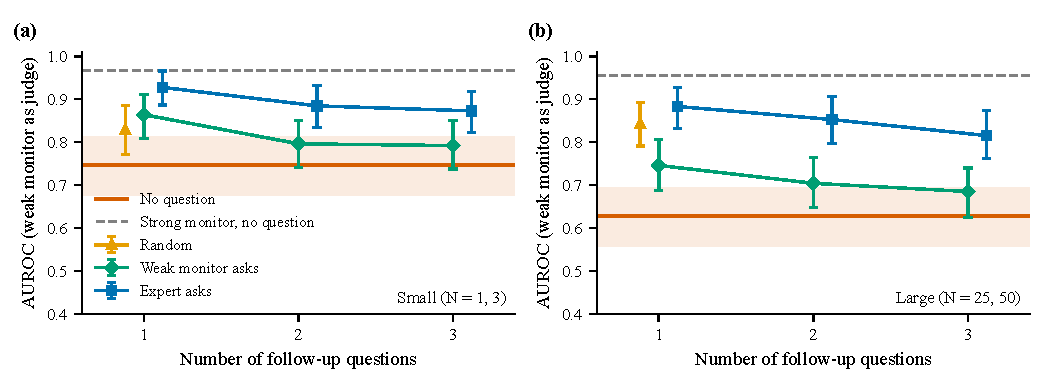
\includegraphics[width=\textwidth]{figures/fig2_followup_rounds.pdf}
\caption{\textbf{More questions do not help; who asks does.} AUROC of the weak monitor as judge after 1--3 follow-up questions, pooled over (a)~small groups ($N{=}1,3$) and (b)~large groups ($N{=}25,50$). Orange line and band: weak monitor with no question. Grey dashed: strong monitor with no question.}
\label{fig:rounds}
\end{figure}

\begin{figure}[h]
\centering
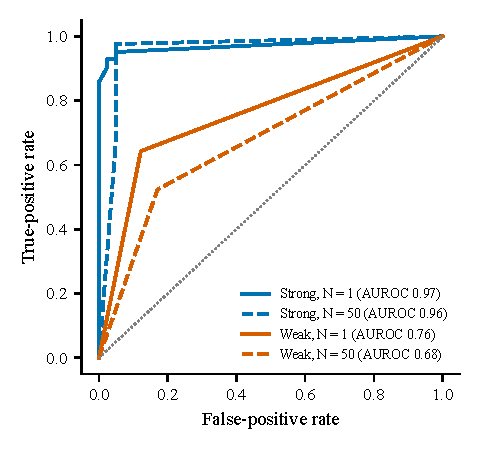
\includegraphics[width=0.45\textwidth]{figures/figS1_roc.pdf}
\caption{ROC curves of the passive weak and strong monitors with 1 and 50 agents in view.}
\end{figure}

\end{document}
